\chapter{Project Definition}
\subsection{Loading data into mysql}
\begin{figure}[H]
\centering
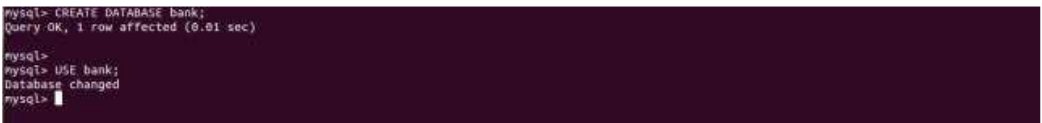
\includegraphics[width=12cm,height=3cm]{1.png}
    \caption{Database Name}
\end{figure}
 
 \section{Creating database bank in mysql:-}
 CREATE DATABASE bank; \newline
 USE bank;

 \newpage
 \section{Creating tables in mysql and inserting the data into mysql tables :-}
 \subsection{Creating table loan\_info}
 CREATE TABLE loan info (loan\_id int,user\_id int,last\_payment\_date DATE,payment\_installation DOUBLE,date\_payable DATE);
 
\begin{figure}[H]
\centering
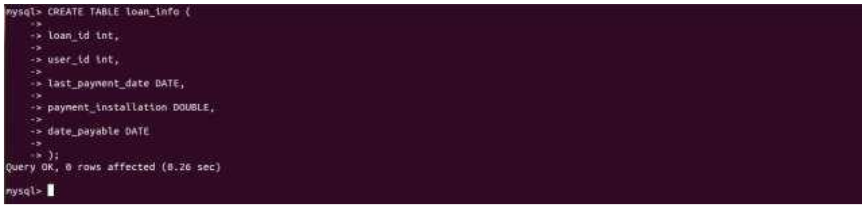
\includegraphics[width=12cm,height=3cm]{table2.png}
    \caption{loan\_info}
\end{figure}

\subsection{Inserting data into loan\_info table}
insert into loan\_info values(1234,5678,'2017-02-20',509,'2017-03-20');\newline
insert into loan\_info values(1243,5687,'2016-02-18',9087,'2016-03-18');\newline
insert into loan\_info values(1324,5786,'2017-03-01',8976,'2017-04-01');\newline
insert into loan\_info values(4312,8976,'2017-01-18',9087,'2017-02-18');\newline
\begin{figure}[H]
\centering
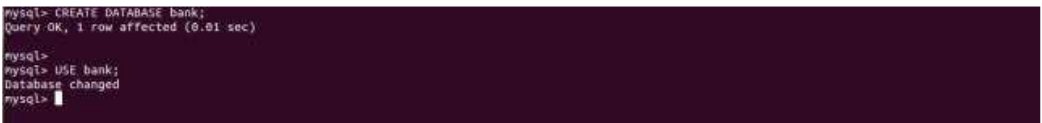
\includegraphics[width=12cm,height=3cm]{1.png}
    \caption{loan\_info}
\end{figure}
   \subsection{Creating table credit\_card\_info}
   CREATE TABLE credit\_card\_info \newline
( \newline
cc\_number bigint, \newline
user\_id int, \newline
maximum\_credit DOUBLE, \newline
outstanding\_balance DOUBLE, \newline
due\_date DATE \newline
); \newline
 
 \subsection{Inserting data into the credit\_card\_info table}
 insert into credit\_card\_info values(1234678753672899,1234,50000,35000,'2017-03-22');\newline insert
into credit\_card\_info values(1234678753672900,1243,500000,500000,'2017-03-12');\newline insert
into credit\_card\_info values(1234678753672902,1324,15000,12000,'2017-03-09');\newline insert into
credit\_card\_info values(1234678753672908,4312,60000,60000,'2017-02-16');\newline

\subsection{Checking the data in credit\_card\_info table}
select * from credit\_card\_info; \newline

\begin{figure}[H]
\centering
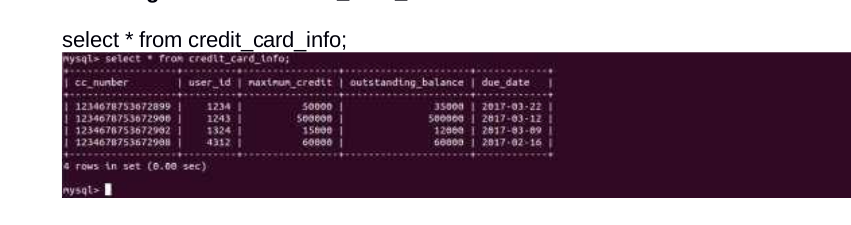
\includegraphics[width=12cm,height=3cm]{creditcard.png}
    \caption{creditcard\_info}
\end{figure}




\subsection{Creating table shares\_info}
CREATE TABLE shares\_info \newline
( \newline
share\_id varchar(10), \newline
company\_name varchar(20), \newline
gmt\_timestamp bigint, \newline
share\_price DOUBLE \newline
); \newline

\subsection{Inserting data into shares\_info table}
insert into shares\_info values('S102',"MyCorp",1488412702,100);\newline
insert into shares\_info values('S102',"MyCorp",1488411802,110);\newline
insert into shares\_info values('S102',"MyCorp",1488411902,90);\newline
insert into shares\_info values('S102',"MyCorp",1488412502,80);\newline
insert into shares\_info values('S102',"MyCorp",1488411502,120);\newline

\subsection{Checking the data in shares\_info table}
select * from shares\_info; \newline
commit; \newline

\begin{figure}[H]
\centering
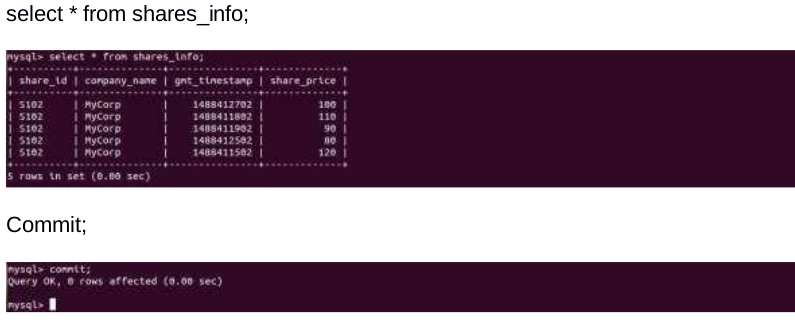
\includegraphics[width=12cm,height=3cm]{sharedinfor.png}
    \caption{shared\_info}
\end{figure}


\section{Exporting data from Mysql to HDFS using sqoop}

Now we have data in mysql. We need to export this data into HDFS. We will do it using sqoop.\newline
For exporting data into HDFS we will first create an user in mysql.\newline
CREATE USER 'myuser'@'localhost' IDENTIFIED BY \newline
'myuser'; grant all on *.* to 'myuser'@'localhost' with grant \newline
option; flush privileges; \newline
commit; \newline    
Now let's transfer these tables into HDFS by writing sqoop jobs.\newline
We will protect our mysql password by saving the password in a file.\newline
echo -n "myuser"\>>sqoop\_mysql\_passwrd\newline

You need to use the option -n. Otherwise, a new line will be created unknowingly and while \newline
reading the password, Sqoop throws an error Access Denied for User.\newline

/* \newline
Sqoop job to transfer data in loan\_info table \newline
Create a directory in HDFS loan\_info\_stg to store the table data \newline
hadoop fs -mkdir /bank \newline
hadoop fs -mkdir /bank/loan\_info\_stg \newline
Above step is not required while performing normal import. \newline
\subsection{Creating sqoop job for sqoop\_loan\_info}
sqoop job --create sqoop\_loan\_info -- import --connect \newline jdbc:mysql://localhost/bank \newline
--username \newline
myuser \newline
--table \newline
loan\_info  \newline
--password-file  \newline
file:///home/santosh/sqoop\_mysql\_passwrd --target-dir  \newline /bank/loan\_info\_stg -m1  \newline
sqoop job --list  \newline

\subsection{Executing the sqoop job sqoop\_loan\_info}

sqoop job --exec sqoop\_loan\_info \newline

Sqoop job to transfer data in credit\_card\_info table \newline

\subsection{Create a directory in HDFS for storing credit\_card\_info table data}

hadoop fs -mkdir /bank/credit\_card\_info\_stg

\subsection{Creating sqoop job credit\_card\_info}

sqoop job --create sqoop\_credit\_card\_info -- import --connect \newline
jdbc:mysql://localhost/bank -- \newline
username myuser --table credit\_card\_info --password-file\newline
\textbf{file:///home/santosh/sqoop\_mysql\_passwrd --target-dir /bank/credit\_card\_info\_stg -m} 1
sqoop job --list

\subsection{Executing the sqoop job sqoop\_loan\_info}
sqoop job --exec sqoop\_loan\_info

\subsection{Sqoop job to transfer data in shares\_info\_table}
\subsubsection{Creating HDFS directory to store shares\_info table data}
hadoop fs -mkdir /bank/shares\_info\_stg
\subsubsection{Creating sqoop job shares\_info}
sqoop job --create sqoop\_shares\_info -- myuser --table shares\_info --password-file \newline file:///home/santosh/sqoop\_mysql\_passwrd
/bank/shares\_info\_stg -m 1
sqoop job
\subsubsection{Executing sqoop\_job shares\_info}
sqoop job --exec sqoop\_shares\_info
--list
\section{Creating external tables in hive}
\subsection{Create database}
CREATE DATABASE bank; \newline
USE bank;
\subsection{Creating table loan\_info\_stg}
As this table is an external table, we just need to give the \newline location of the data.\newline
CREATE EXTERNAL TABLE loan\_info\_stg ( \newline
Loan\_id int,\newline
User\id int,\newline
last\_payment\_date string,\newline
payment\_installation double,\newline
Date\_payable string\newline
) ROW FORMAT DELIMITED FIELDS TERMINATED BY\newline
',' LOCATION '/bank/loan\_info\_stg';\newline

\subsection{Creating table credit\_card\_info\_stg}

CREATE EXTERNAL TABLE \newline
credit\_card\_info\_stg ( \newline
cc\_number string, \newline
user\_id int, \newline
maximum\_credit double, \newline
outstanding\_balance double, \newline
due\_date string \newline
) ROW FORMAT DELIMITED FIELDS TERMINATED BY \newline
',' LOCATION '/bank/credit\_card\_info\_stg'; \newline

\subsection{Creating table shares\_info\_stg}

CREATE EXTERNAL TABLE shares\_info\_stg \newline
( \newline
Share\_id string, \newline
Company\_name string, \newline
Gmt\_timestamp bigint, \newline
Share\_price double \newline
) ROW FORMAT DELIMITED FIELDS TERMINATED BY \newline
',' LOCATION '/bank/shares\_info\_stg'; \newline

\subsection{Creating core tables and loading the data into the core tables from stg tables}
Adding the udf into hive shell. \newline
CREATE TEMPORARY FUNCTION encrypt AS 'encryption.AESencrypt';\newline
CREATE TEMPORARY FUNCTION decrypt AS 'encryption.AESdecrypt';\newline
\subsection{Creating loan\_info table}
CREATE TABLE loan\_info ( \newline
Loan\_id string, \newline
User\_id string, \newline
last\_payment\_date string, \newline
payment\_installation string, \newline
Date\_payable string \newline
) STORED AS ORC; \newline

\subsection{Inserting data into loan\_info table}

INSERT INTO TABLE loan\_info \newline
SELECT encrypt(Loan\_id), \newline
encrypt(User\_id), \newline
encrypt(last\_payment\_date), \newline
encrypt(payment\_installation), \newline
encrypt(Date\_payable) \newline
FROM loan\_info\_stg; \newline

\subsection{Creating credit\_card\_info table}
CREATE TABLE credit\_card\_info \newline
( \newline
cc\_number string, \newline
user\_id string, \newline
maximum\_credit string, \newline
outstanding\_balance string, \newline
due\_date string \newline
) STORED AS ORC; \newline

\subsection{Inserting data into credit\_card\_info table}
INSERT INTO TABLE credit\_card\_info \newline
SELECT encrypt(cc\_number), \newline
encrypt(User\_id), \newline
encrypt(maximum\_credit), \newline
encrypt(outstanding\_balance), \newline
encrypt(due\_date) \newline
FROM credit\_card\_info\_stg; \newline

\subsection{Creating shares\_info table}
CREATE TABLE shares\_info \newline
( \newline
Share\_id string, \newline
Company\_name string, \newline
Gmt\_timestamp string, \newline
Share\_price string \newline
) STORED AS ORC;\newline

\subsection{Inserting data into shares\_info table}
INSERT INTO TABLE shares\_info \newline
SELECT encrypt(Share\_id), \newline
encrypt(Company\_name), \newline
encrypt(Gmt\_timestamp), \newline
encrypt(Share\\price) \newline
FROM shares\_info\_stg; \newline

\subsection{Checking the data in the three tables}
As the data is bank data, we have encrypted the data.\newline
You can truncate the data from stg tables.\newline

\section{Analysis}
\subsection{Decrypting the data for analysis}
CREATE TEMPORARY FUNCTION encrypt AS 'encryption.AESencrypt';\newline
CREATE TEMPORARY FUNCTION decrypt AS 'encryption.AESdecrypt';\newline
CREATE TEMPORARY FUNCTION max\_profit AS 'maxprofit.MaxProfit';\newline
SET hive.auto.convert.join=false;\newline

\subsection{Find out the list of users who have at least 2 loan instalments pending.}
SELECT decrypt(user\_id) \newline
FROM loa\_info \newline
WHERE datediff(from\_unixtime(unix\_timestamp(), 'yyyy-MM-dd'), \newline
decrypt(last\_payment\_date)) >= 60; \newline

\subsection{Find the list of users who have a healthy credit card but outstanding loan account.
Healthy credit card means no outstanding balance.}
SELECT decrypt(li.user\_id) \newline
FROM loan\_info li INNER JOIN credit\_card\_info \newline
cci ON decrypt(li.user\_id) = decrypt(cci.user\_id) \newline
WHERE CAST(decrypt(cci.outstanding\_balance) AS double) = 0.0 \newline
AND datediff(from\_unixtime(unix\_timestamp(), 'yyyy-MM-dd'), \newline
decrypt(li.last\_payment\_date) >= 30); \newpage

\subsection{For every share and for every date, find the maximum profit one could have made
on the share. Bear in mind that a share purchase must be before share sell and if share
prices fall throughout the day, maximum possible profit may be negative.}
\begin{verbatim}
SELECT share_id, share_date,
max\profit(collect_list(share_price))
FROM
( 
SELECT decrypt(Share_id) AS share_id,
decrypt(Gmt_timestamp) AS Gmt_timestamp,
from_unixtime(CAST(decrypt(Gmt_timestamp) AS int), 'yyyy-MM-dd')
share_date, CAST (decrypt(Share_price) AS double) AS share_price FROM
shares_info
DISTRIBUTE BY share_id,
from_unixtime(CAST(Gmt_timestamp AS int), 'yyyy-MM-dd')
SORT BY share_id,
CAST(Gmt_timestamp AS int)
) inne GROUP BY share_id, share_date;
\end{verbatim}
\section{Survey data analysis}

We have 3 survery part files. So we will copy the contents into a \newline single file using the below \newline
linux commands. \newline
cd /home/acadgild/survey\_files \newline
cat *.txt > survey\_data \newline
rm *.txt \newline
Now we have the concated data in survey\_data file.\newline
\newpage
\subsection{Creating hive table to load survey\_data}

CREATE TABLE survey\_analysis ( \newline
survey\_date string, \newline
survey\_question string, \newline
Rating int, \newline
user\_id int, \newline
survey\_id string \newline
) \newline
ROW FORMAT DELIMITED  \newline
FIELDS TERMINATED BY ',';  \newline

\subsection{Loading data into survey\_analysis table}

LOAD DATA LOCAL INPATH '/home/acadgild/survey\_files/survey\_data'\newline INTO TABLE \newline
bank.survey\_analysis; \newpage


\section{Result}
\begin{itemize}
    \item The localhost page of Hadoop is shown in figure 16.To access this page, step to be followed:\\
Start Hadoop services form terminal.\\
Enter localhost:50070 in web address of any web browser.\\
from this page user can browse the file system.
\end{itemize}
\begin{figure}[htb]
\centering
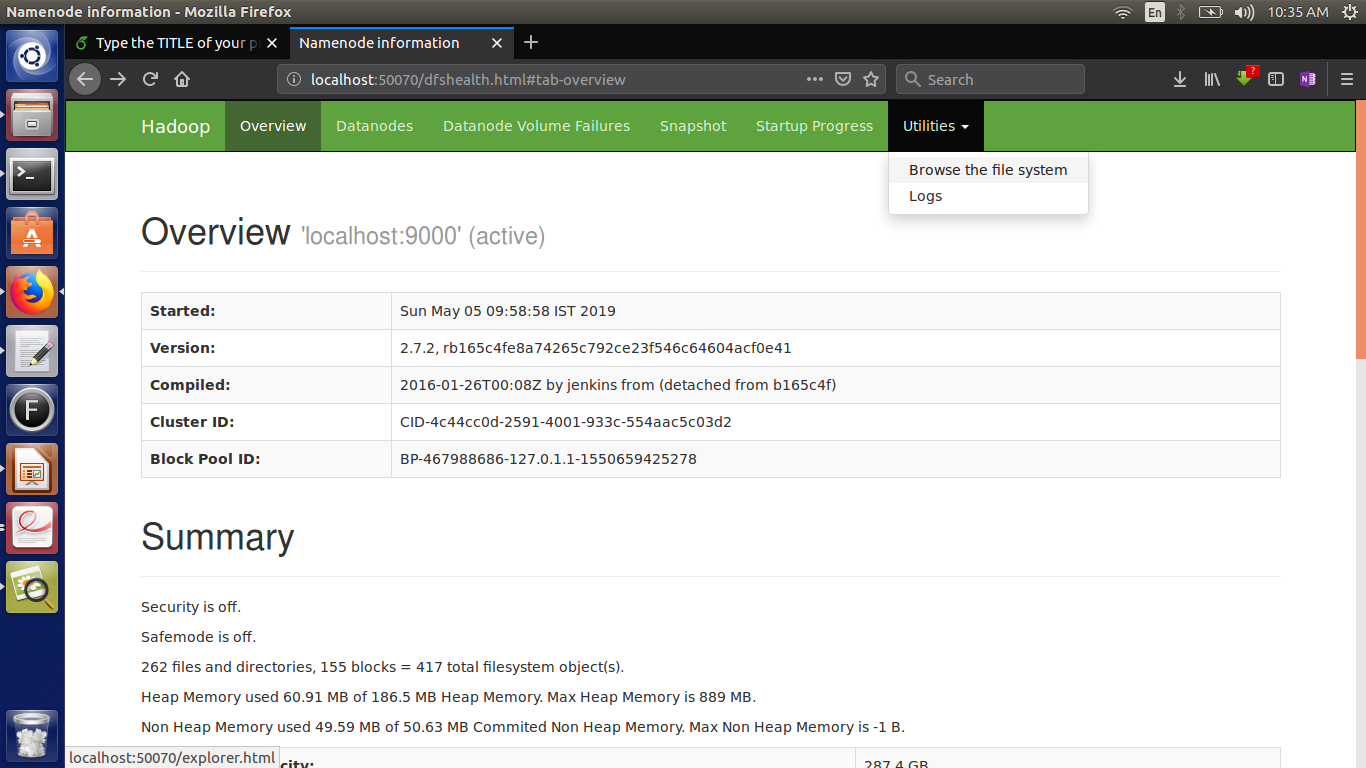
\includegraphics[width=8cm,height=8cm]{1stp.png}
    \caption{Browsing File}
\end{figure} \newpage
\begin{itemize}
    
\item  From browse the file system, User can view screen as shown in figure 17. Now ,User can select Bank related to detail he/she have stored,

\end{itemize}
\begin{figure}[htb]
\centering
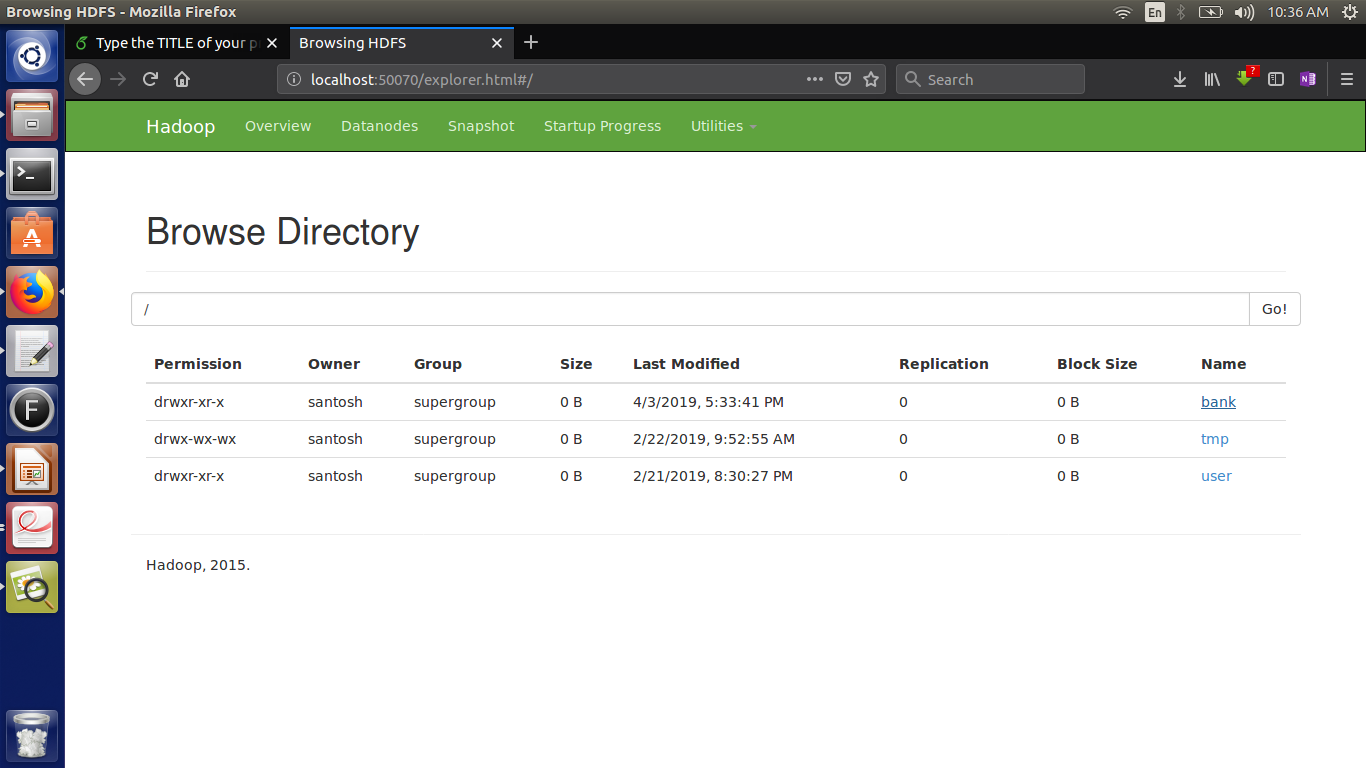
\includegraphics[width=8cm,height=8cm]{2ndp.png}
    \caption{Bank information}
\end{figure} \newpage
\begin{itemize}
    \item 

This diagram represent Credit Card Information means that a credit card is different from a charge card, which requires the balance to be repaid in full each month.In contrast, credit cards allow the consumers to build a continuing balance of debt, subject to interest being charged. A credit card also differs from a cash card, which can be used like currency by the owner of the card. A credit card differs from a charge card also in that a credit card typically involves a third-party entity that pays the seller and is reimbursed by the buyer, whereas a charge card simply defers payment by the buyer until a later date.
\end{itemize}
\begin{figure}[htb]
\centering
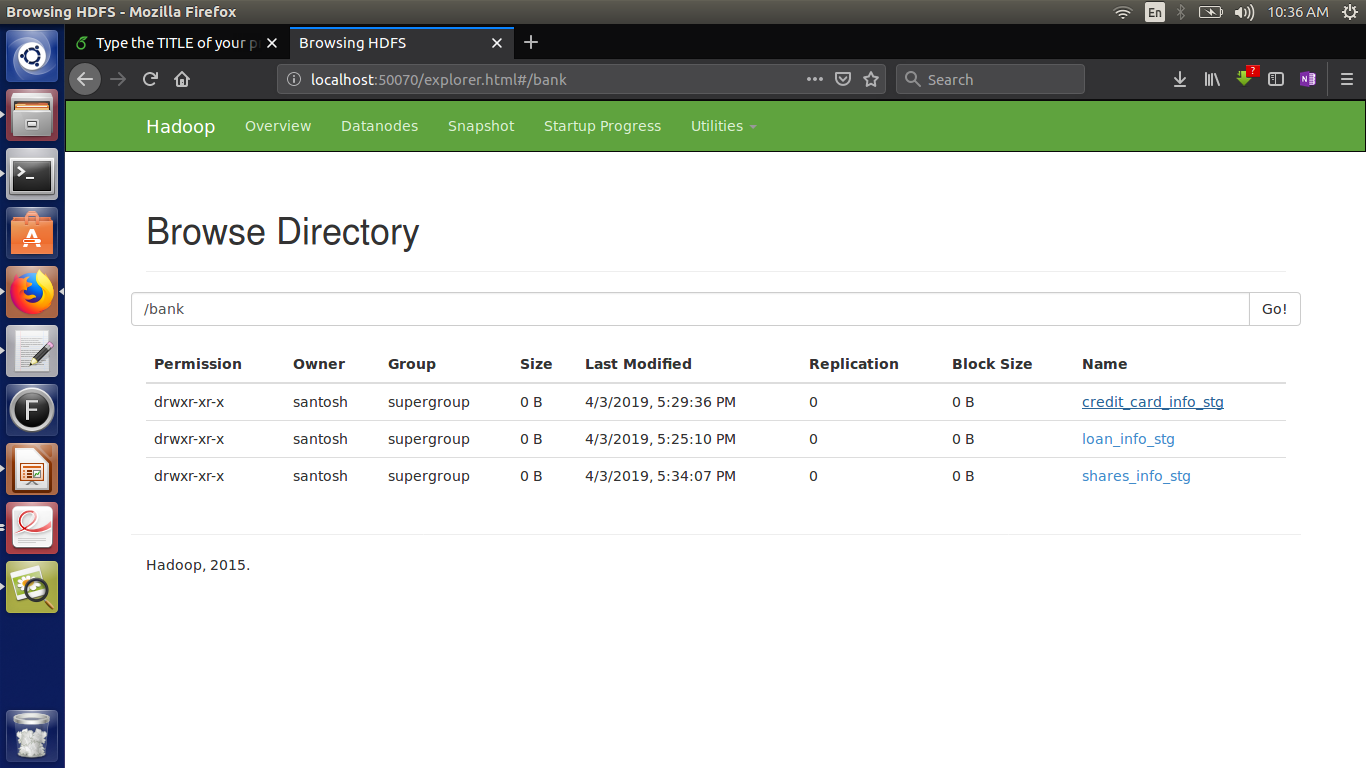
\includegraphics[width=8cm,height=8cm]{3p.png}
    \caption{credit card information}
\end{figure} \newpage
\begin{itemize}
    \item The Credit card information is successfully uploaded.

 
 \end{itemize}
\begin{figure}[htb]
\centering
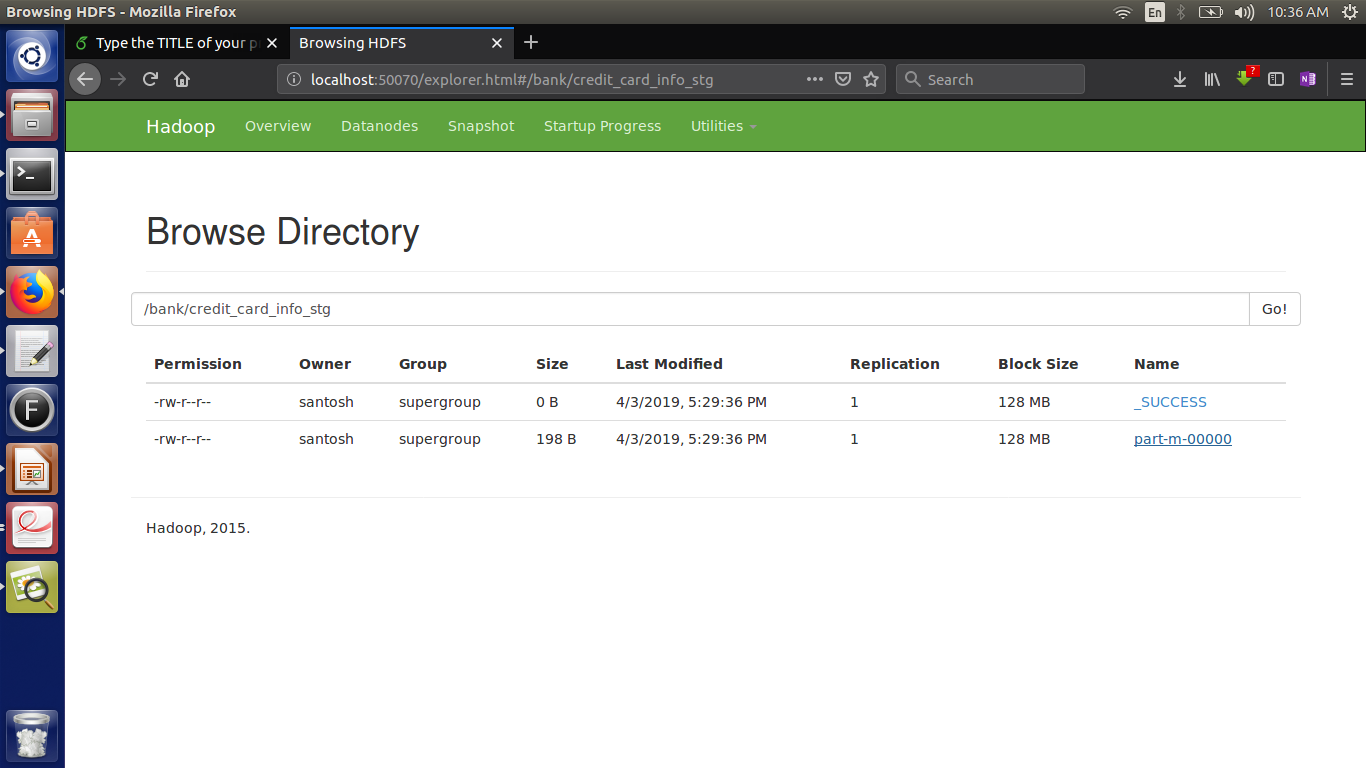
\includegraphics[width=8cm,height=8cm]{4p.png}
    \caption{Browsing Data}
\end{figure} \newpage
\begin{itemize}
    \item After selecting credit card information link user can download data using screen link. This related page is as shown in figure.
\end{itemize}
\begin{figure}[htb]
\centering
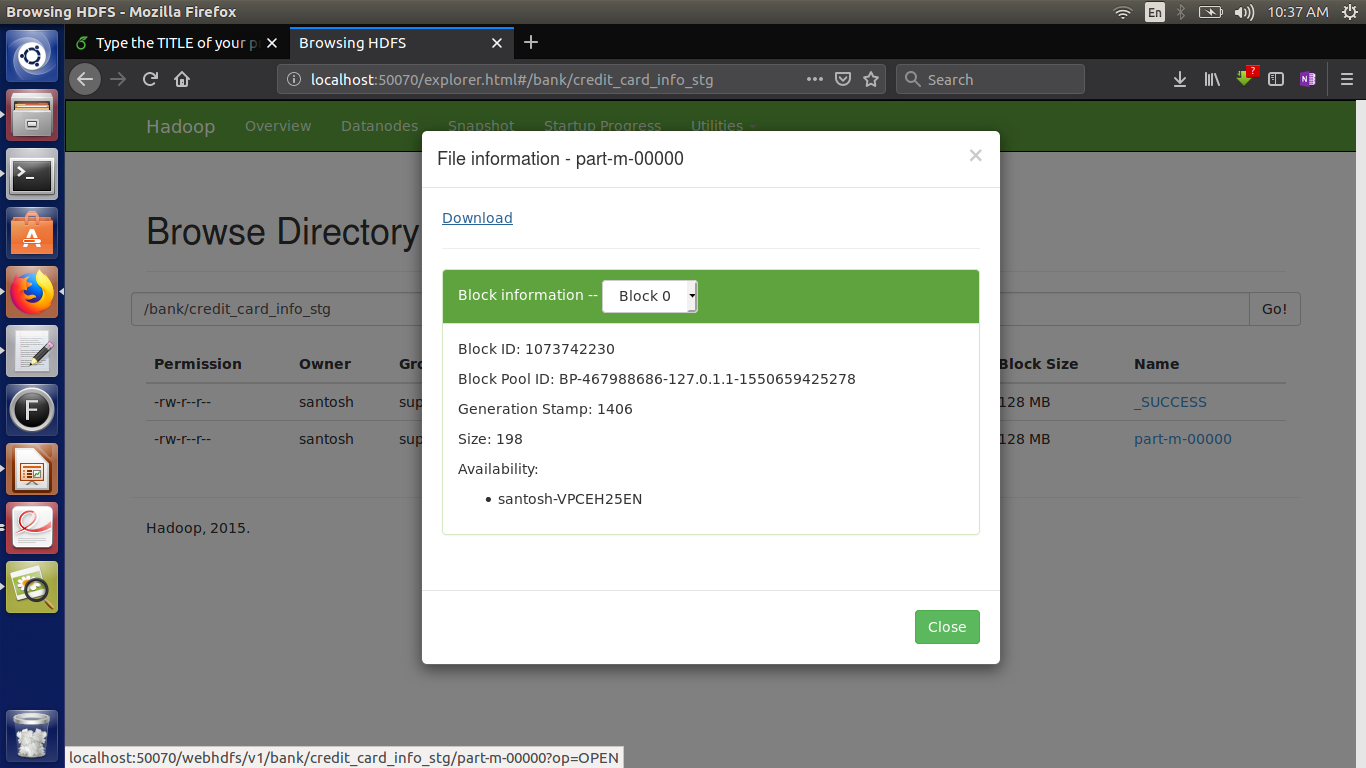
\includegraphics[width=8cm,height=8cm]{5p.png}
    \caption{File Information}
\end{figure} \newpage
\begin{itemize}
    \item After selecting loan information link form Bank, User can download data using success link. the related page is shown in figure.
    \item A loan is the lending of money by one or more individuals, organizations, or other entities to other individuals, organizations etc. The recipient (i.e. the borrower) incurs a debt, and is usually liable to pay interest on that debt until it is repaid, and also to repay the principal amount borrowed. 
\end{itemize}
\begin{figure}[htb]
\centering
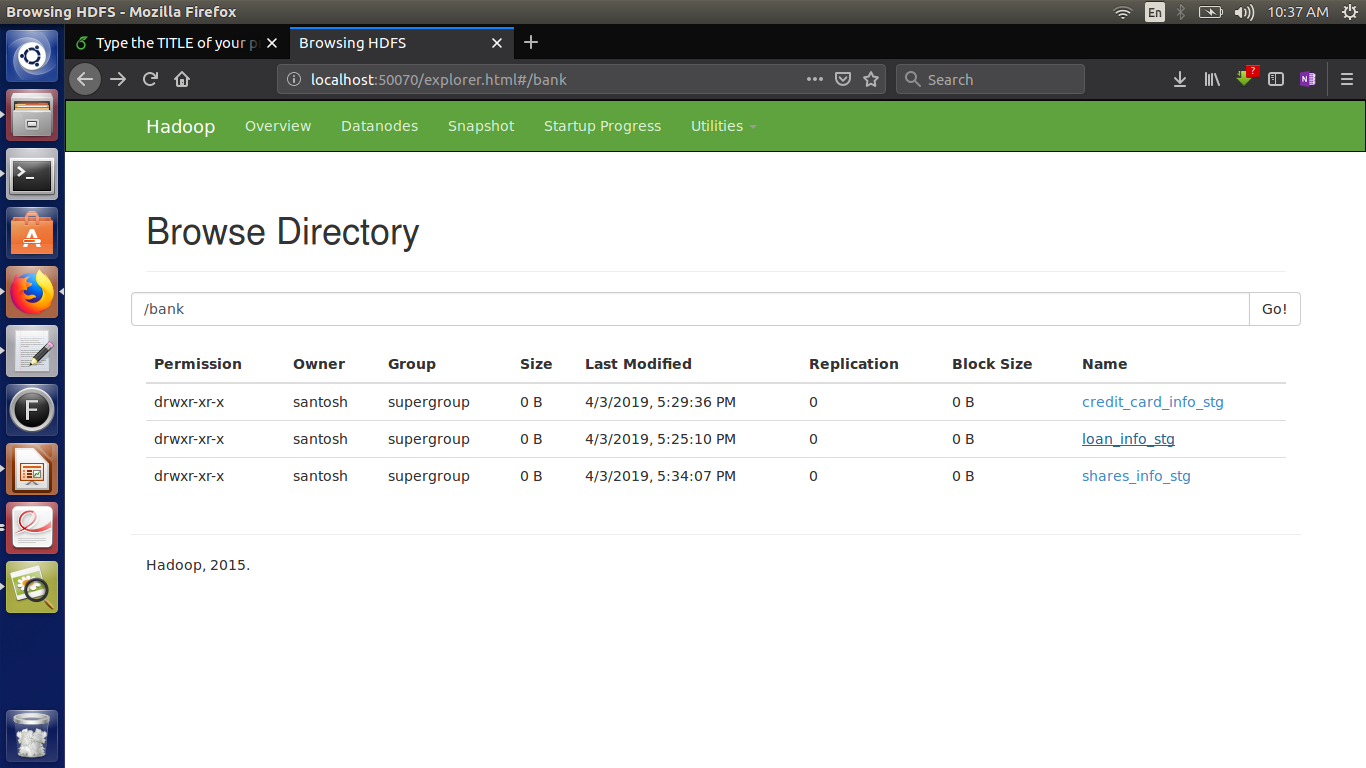
\includegraphics[width=8cm,height=8cm]{6p.png}
    \caption{loan Information}
\end{figure} \newpage

\begin{itemize}
    \item In this section all the data have successfully update.
\end{itemize}
\begin{figure}[htb]
\centering
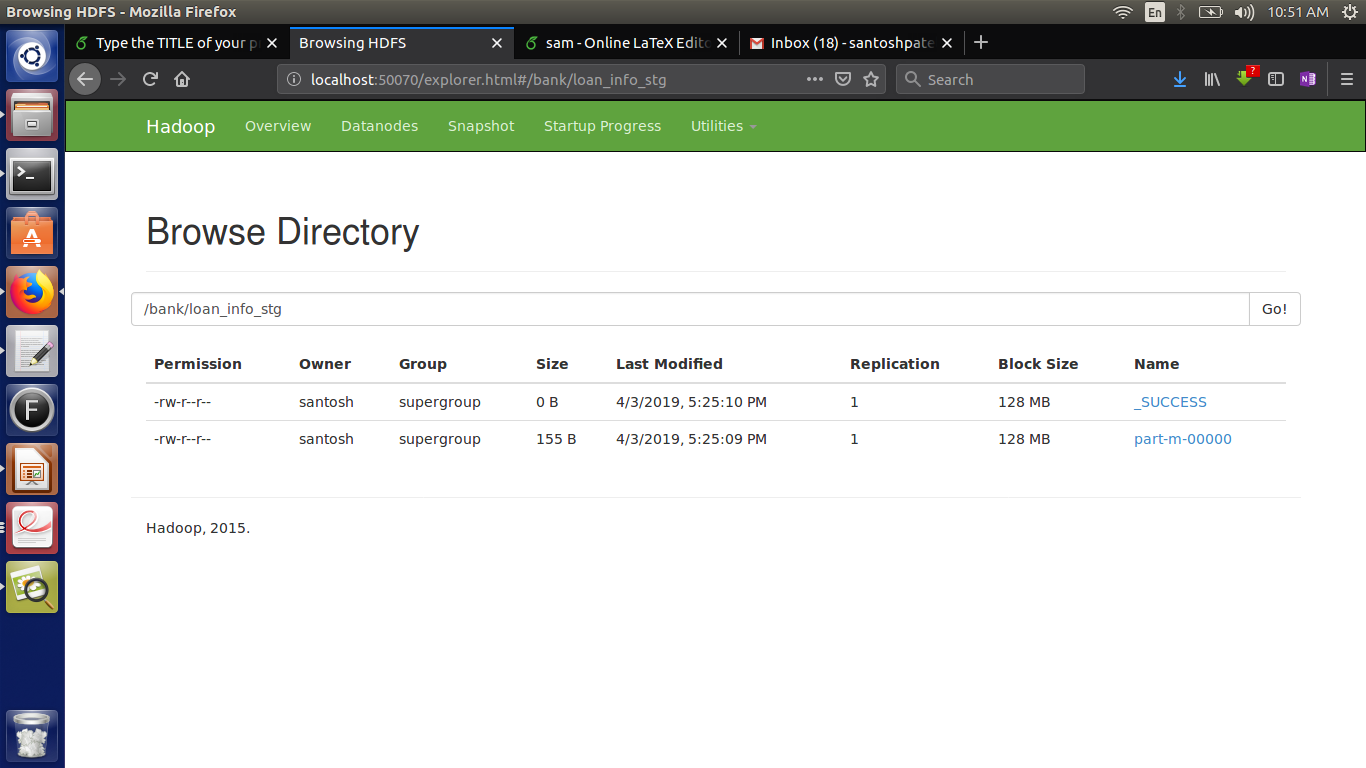
\includegraphics[width=8cm,height=8cm]{7pag.png}
    \caption{File information of loan}
\end{figure} \newpage

\begin{itemize}
    \item The download link appears as shown in figure.
\end{itemize}
\begin{figure}[htb]
\centering
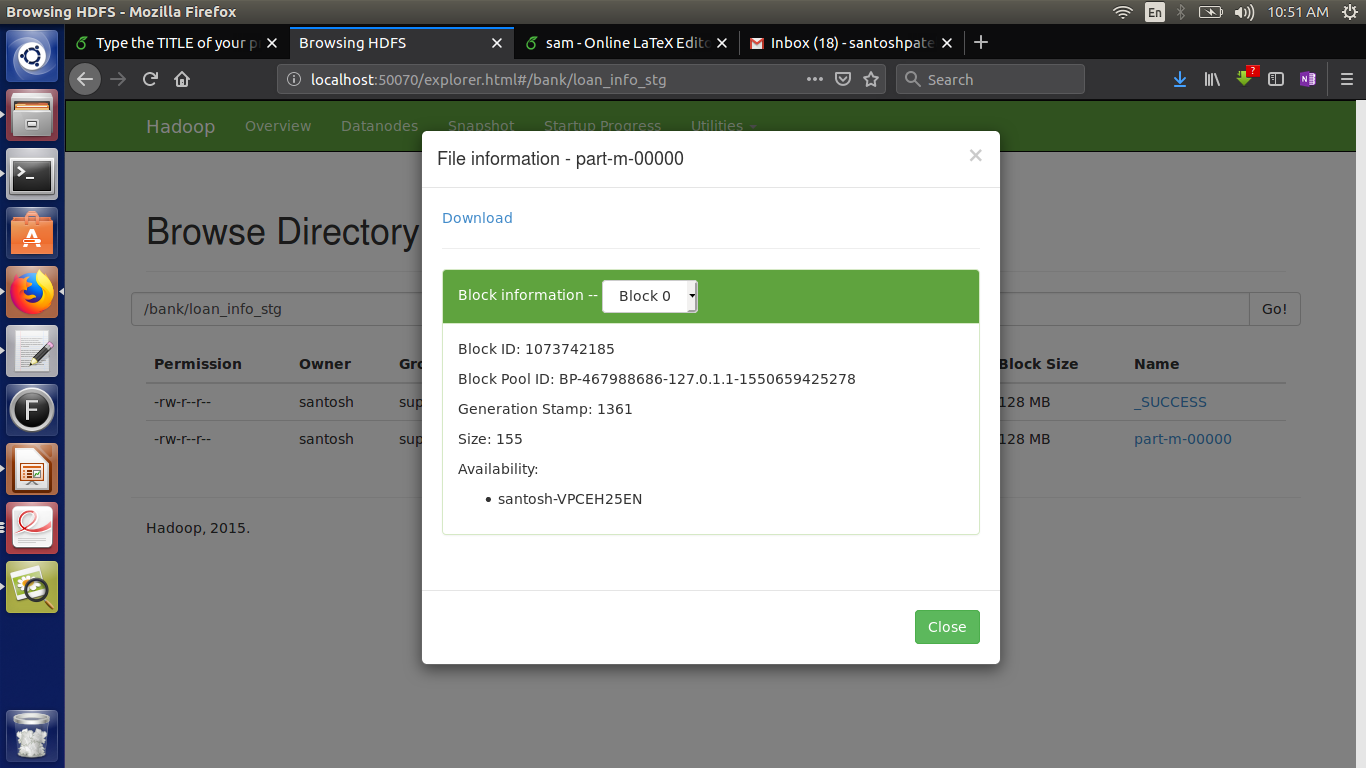
\includegraphics[width=8cm,height=8cm]{8page.png}
    \caption{Browsing File}
\end{figure} \newpage
\begin{itemize}
    \item After the selecting shares information link, User can download data using success link.the related page is shown in figure.
\end{itemize}

\begin{figure}[htb]
\centering
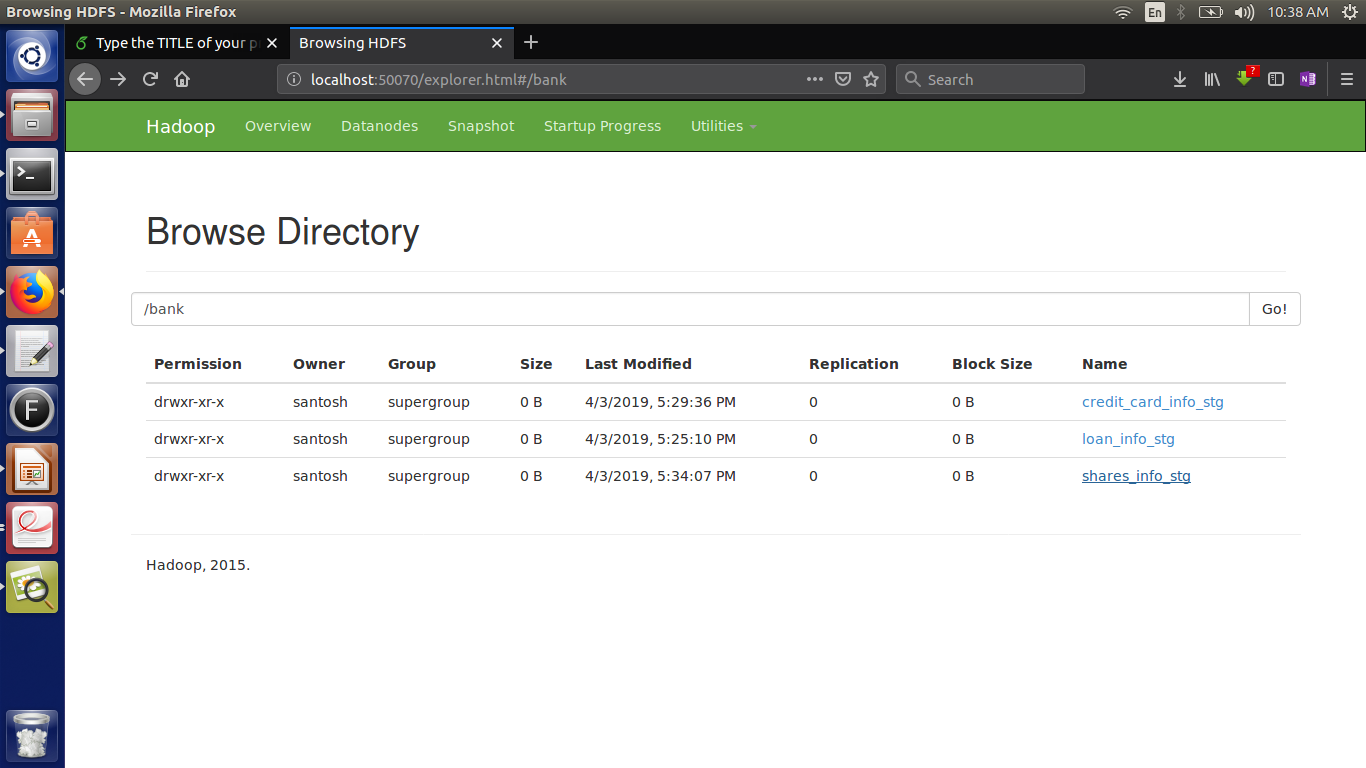
\includegraphics[width=8cm,height=8cm]{9thp.png}
    \caption{Browsing File shares information}
\end{figure} \newpage
\\

\begin{itemize}
    \item All data have been successfully upload.
\end{itemize}
\begin{figure}[htb]
\centering
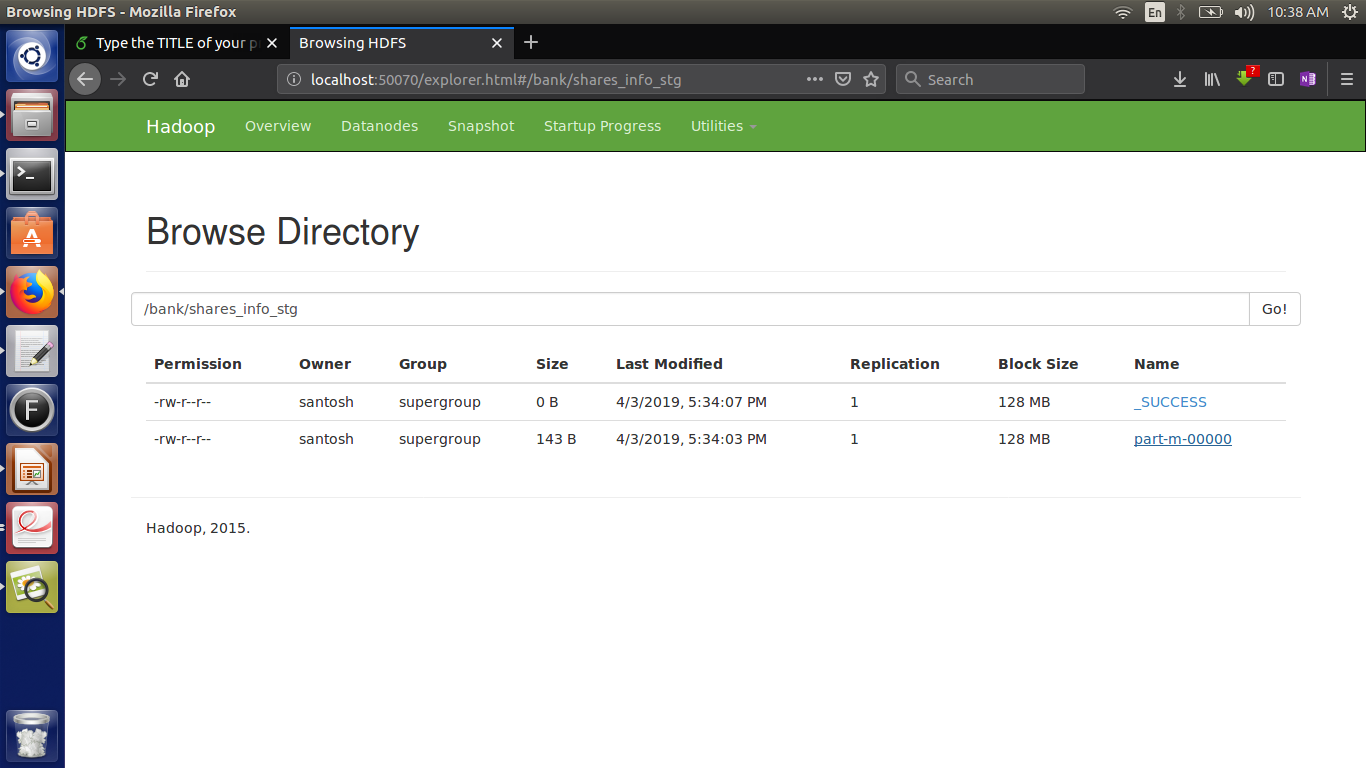
\includegraphics[width=8cm,height=8cm]{10p.png}
    \caption{shares information}
\end{figure} \newpage


